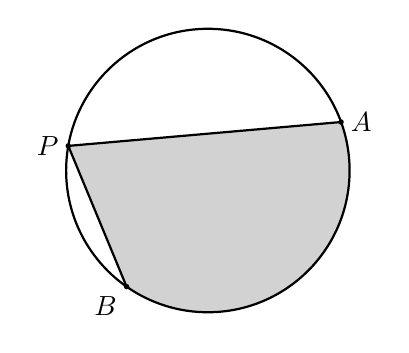
\begin{tikzpicture}[line cap=round,line join=round,scale=0.9]
\usetikzlibrary{calc}

\def\R{2.0}
\def\angA{20}
\def\angP{170}
\def\angB{235}

\coordinate (O) at (0,0);
\coordinate (A) at ({\R*cos(\angA)},{\R*sin(\angA)});
\coordinate (P) at ({\R*cos(\angP)},{\R*sin(\angP)});
\coordinate (B) at ({\R*cos(\angB)},{\R*sin(\angB)});

% 阴影：P--A--(沿不经过P的弧AB)--B--P
\path[fill=gray!35]
  (P) -- (A)
  arc[start angle=\angA,end angle=\angB-360,radius=\R]
  -- (P) -- cycle;

% 圆周
\draw[thick] (O) circle (\R);

% 弦
\draw[thick] (P)--(A);
\draw[thick] (P)--(B);

% 标注
\fill (A) circle (1.1pt) node[right] {$A$};
\fill (P) circle (1.1pt) node[left] {$P$};
\fill (B) circle (1.1pt) node[below left] {$B$};

\end{tikzpicture}